\documentclass[aspectratio=169, 10pt]{beamer}

% -----------------------------------------------------------------------------
% Theme & Typography Setup
% -----------------------------------------------------------------------------
\usetheme{Madrid}
\usefonttheme{professionalfonts}

\usepackage[english]{babel}
\usepackage{amsmath,amsfonts,amssymb}
\usepackage{booktabs}
\usepackage{graphicx}
\usepackage{colortbl}
\usepackage{hyperref}

% -----------------------------------------------------------------------------
% Clean, Modern Color Palette
% -----------------------------------------------------------------------------
\definecolor{NavyBlue}{RGB}{14, 43, 82}
\definecolor{Teal}{RGB}{18, 128, 133}
\definecolor{Crimson}{RGB}{200, 35, 45}
\definecolor{SoftGray}{RGB}{248, 249, 251}
\definecolor{DarkSlate}{RGB}{40, 45, 50}
\definecolor{LightTeal}{RGB}{236, 248, 248}

\setbeamercolor{structure}{fg=NavyBlue}
\setbeamercolor{palette primary}{bg=NavyBlue,fg=white}
\setbeamercolor{palette secondary}{bg=Teal,fg=white}
\setbeamercolor{palette tertiary}{bg=DarkSlate,fg=white}
\setbeamercolor{frametitle}{bg=NavyBlue,fg=white}
\setbeamercolor{title}{bg=NavyBlue,fg=white}

% Clean Block Styling
\setbeamercolor{block title}{bg=NavyBlue,fg=white}
\setbeamercolor{block body}{bg=SoftGray,fg=DarkSlate}
\setbeamercolor{block title example}{bg=Teal,fg=white}
\setbeamercolor{block body example}{bg=LightTeal,fg=DarkSlate}
\setbeamercolor{block title alerted}{bg=Crimson,fg=white}
\setbeamercolor{block body alerted}{bg=SoftGray,fg=DarkSlate}

\setbeamertemplate{blocks}[rounded][shadow=false]
\setbeamertemplate{items}[circle]
\setbeamertemplate{navigation symbols}{}

% Uncluttered Footer
\setbeamertemplate{footline}{
  \leavevmode%
  \hbox{%
  \begin{beamercolorbox}[wd=.35\paperwidth,ht=2.4ex,dp=1ex,left,leftskip=2ex]{author in head/foot}%
    \usebeamerfont{author in head/foot}\textbf{Amrita Vishwa Vidyapeetham}
  \end{beamercolorbox}%
  \begin{beamercolorbox}[wd=.40\paperwidth,ht=2.4ex,dp=1ex,center]{title in head/foot}%
    \usebeamerfont{title in head/foot}GlycoTwin: T2D Digital Twin
  \end{beamercolorbox}%
  \begin{beamercolorbox}[wd=.25\paperwidth,ht=2.4ex,dp=1ex,right,rightskip=2ex]{date in head/foot}%
    \usebeamerfont{date in head/foot}\insertframenumber{} / \inserttotalframenumber
  \end{beamercolorbox}}%
  \vskip0pt%
}

\graphicspath{{images/}{./}}

% -----------------------------------------------------------------------------
% Title Slide Metadata
% -----------------------------------------------------------------------------
\title[\textbf{GlycoTwin: T2D Digital Twin}]{\textbf{Personalized Multi-Modal Digital Twin for Type 2 Diabetes Management}}
\subtitle{Continuous Glucose Forecasting \& Causal "What-If" Simulation}

\author[Divagar S, Abhishek Pandey, Prem]{
  \textbf{Divagar S} \quad $\vert$ \quad \textbf{Abhishek Pandey} \quad $\vert$ \quad \textbf{Prem}
}

\institute[Amrita Vishwa Vidyapeetham]{
  \vspace{-0.15cm}
  {\small \textbf{Project Guide:} \textbf{Dr. Keerthika K}, Assistant Professor}\\[0.1cm]
  Department of Artificial Intelligence, School of Computing\\
  Amrita Vishwa Vidyapeetham, Coimbatore Campus
}

\date{October 27, 2026}

% =============================================================================
% SLIDES
% =============================================================================
\begin{document}

% -----------------------------------------------------------------------------
% Slide 1: Title
% -----------------------------------------------------------------------------
\begin{frame}[plain]
  \begin{center}
    
\includegraphics[height=1.15cm]{images/univA.png}\\[0.15cm]
    {\scriptsize \textbf{DEPARTMENT OF ARTIFICIAL INTELLIGENCE --- AMRITA VISHWA VIDYAPEETHAM}}\\[0.15cm]
    \hrule height 1pt
    \vspace{0.25cm}
    {\large \textbf{\color{NavyBlue} Personalized Multi-Modal Digital Twin for Type 2 Diabetes}}\\[0.1cm]
    {\footnotesize \color{Teal} Postprandial Glucose Forecasting and Causal Lifestyle Simulation}\\[0.25cm]
    \hrule height 0.5pt
    \vspace{0.3cm}
    
    \begin{columns}[c]
      \begin{column}{0.52\textwidth}
        \scriptsize
        \textbf{Students:}\\
        $\bullet$ \textbf{Divagar S} (CB.SC.U4AIE23223)\\
        $\bullet$ \textbf{Abhishek Pandey} (CB.SC.U4AIE23205)\\
        $\bullet$ \textbf{Prem} (CB.SC.U4AIE23241)
      \end{column}
      \begin{column}{0.45\textwidth}
        \scriptsize
        \textbf{Supervisor:}\\
        \textbf{Dr. Keerthika K}\\
        Assistant Professor\\
        Dept. of Artificial Intelligence
      \end{column}
    \end{columns}
    
    \vspace{0.35cm}
    {\tiny B.Tech Major Project Thesis Defense $\cdot$ October 2026}
  \end{center}
\end{frame}

% -----------------------------------------------------------------------------
% Slide 2: Outline
% -----------------------------------------------------------------------------
\begin{frame}{Presentation Outline}
  \begin{columns}[c]
    \begin{column}{0.48\textwidth}
      \begin{block}{Part I: Motivation \& Modeling}
        \begin{itemize}\setlength{\itemsep}{0.6em}
          \item Clinical Motivation \& Research Gap
          \item Synchronized Multi-Modal Dataset
          \item Gut Microbiome Latent Learning ($\beta$-VAE)
          \item TransformerForecaster Architecture
        \end{itemize}
      \end{block}
    \end{column}
    
    \begin{column}{0.48\textwidth}
      \begin{block}{Part II: Results, Simulation \& App}
        \begin{itemize}\setlength{\itemsep}{0.6em}
          \item Experimental Protocol \& Baselines
          \item Benchmark Results \& Clinical Safety
          \item Causal "What-If" Simulation Engine
          \item Mobile Web App \& Conclusion
        \end{itemize}
      \end{block}
    \end{column}
  \end{columns}
\end{frame}

% -----------------------------------------------------------------------------
% Slide 3: Clinical Motivation
% -----------------------------------------------------------------------------
\begin{frame}{Motivation: Why "One-Size-Fits-All" Diets Fail}
  \begin{columns}[c]
    \begin{column}{0.55\textwidth}
      \begin{itemize}\setlength{\itemsep}{0.8em}
        \item \textbf{Diabetes Epidemic:} Affects over 537 million people worldwide; post-meal sugar spikes drive severe complications.
        \item \textbf{High Personal Variation:} Clinical trials show two people eating the \emph{exact same meal} can have completely opposite glucose spikes.
        \item \textbf{Complex Interactions:} Blood sugar response is shaped by:
        \begin{itemize}\setlength{\itemsep}{0.3em}
          \item Gut microbiome composition
          \item Physical activity \& pre-meal momentum
          \item Baseline insulin resistance (HOMA-IR)
        \end{itemize}
      \end{itemize}
    \end{column}
    
    \begin{column}{0.42\textwidth}
      \begin{exampleblock}{The Objective}
        Move from generic food guidelines to a \textbf{Personalized Digital Twin} that forecasts glucose curves \emph{before} a meal is eaten.
      \end{exampleblock}
    \end{column}
  \end{columns}
\end{frame}

% -----------------------------------------------------------------------------
% Slide 4: Limitations of Current CGMs
% -----------------------------------------------------------------------------
\begin{frame}{Limitations of Existing Continuous Glucose Monitoring}
  \begin{columns}[c]
    \begin{column}{0.48\textwidth}
      \begin{block}{1. Reactive, Not Proactive}
        \begin{itemize}\setlength{\itemsep}{0.4em}
          \item Alerts trigger \textbf{after} sugar crosses 180 mg/dL.
          \item Food is already digested; patients cannot undo the spike retrospectively.
        \end{itemize}
      \end{block}
      
      \vspace{0.2cm}
      \begin{block}{2. Isolated Sensor Readings}
        \begin{itemize}\setlength{\itemsep}{0.4em}
          \item CGMs track glucose without connecting meal nutrients, smartwatch fitness, or blood labs.
        \end{itemize}
      \end{block}
    \end{column}
    
    \begin{column}{0.48\textwidth}
      \begin{block}{3. Gut Microbiome is Ignored}
        \begin{itemize}\setlength{\itemsep}{0.4em}
          \item 1,900+ bacterial taxa are hard to model in small patient cohorts.
          \item Standard PCA fails on sparse binary bacterial presence data.
        \end{itemize}
      \end{block}
      
      \vspace{0.2cm}
      \begin{alertblock}{Baseline Collapse in Standard ML}
        Standard models collapse to the average ($\approx 120$ mg/dL), completely flattening spikes.
      \end{alertblock}
    \end{column}
  \end{columns}
\end{frame}

% -----------------------------------------------------------------------------
% Slide 5: Problem Statement & Objectives
% -----------------------------------------------------------------------------
\begin{frame}{Problem Statement \& Research Objectives}
  \begin{block}{Problem Statement}
    To build a personalized multi-modal digital twin that predicts continuous 2-hour post-meal glucose curves and enables "what-if" lifestyle simulations before eating.
  \end{block}
  
  \vspace{0.3cm}
  \textbf{Key Objectives:}
  \begin{enumerate}\setlength{\itemsep}{0.5em}
    \item \textbf{Data Pipeline:} Synchronize dual CGM, smartwatch, diet, lab, and microbiome data.
    \item \textbf{Microbiome $\beta$-VAE:} Compress 1,979 bacterial taxa into 8 meaningful latent features.
    \item \textbf{TransformerForecaster:} Build an attention model predicting 120-min trajectories using a relative delta formulation ($\Delta G$).
    \item \textbf{Unseen Validation:} Test on completely unseen participants with clinical safety checks.
    \item \textbf{Mobile Simulation:} Deploy an interactive web app for real-time pre-meal decisions.
  \end{enumerate}
\end{frame}

% -----------------------------------------------------------------------------
% Slide 6: Dataset Synchronization
% -----------------------------------------------------------------------------
\begin{frame}{Synchronized Multi-Modal Dataset (CGMacros)}
  \begin{columns}[c]
    \begin{column}{0.50\textwidth}
      \begin{itemize}\setlength{\itemsep}{0.6em}
        \item \textbf{Cohort:} 45 participants (healthy, pre-diabetic, T2D) with \textbf{1,633 logged meals}.
        \item \textbf{Dynamic Streams (60 min pre-meal):}
        \begin{itemize}\setlength{\itemsep}{0.2em}
          \item Dual CGM (Libre \& Dexcom G6 at 1-min intervals)
          \item Fitbit Heart Rate \& METs physical exertion
        \end{itemize}
        \item \textbf{Static Covariates (61 features):}
        \begin{itemize}\setlength{\itemsep}{0.2em}
          \item Meal: Carbs, Fiber, Protein, Fat, Calories
          \item Clinical: Fasting glucose, HbA1c, HOMA-IR, Lipids
          \item Gut: 8 latent values from $\beta$-VAE
        \end{itemize}
      \end{itemize}
    \end{column}
    
    \begin{column}{0.48\textwidth}
      \centering
      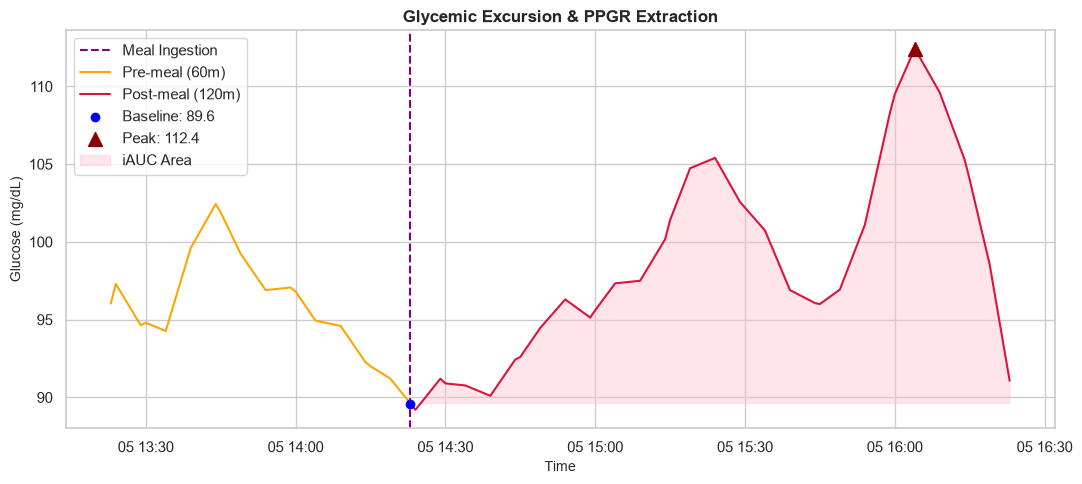
\includegraphics[width=\linewidth,height=0.62\textheight,keepaspectratio]{images/glycemic_excursion_and_ppgr_extraction.png}\\[0.1cm]
      {\scriptsize \color{DarkSlate} Pre-meal 60-min window $\to$ 120-min post-meal forecast}
    \end{column}
  \end{columns}
\end{frame}

% -----------------------------------------------------------------------------
% Slide 7: Microbiome Latent Modeling (Beta-VAE)
% -----------------------------------------------------------------------------
\begin{frame}{Gut Microbiome Representation Learning ($\beta$-VAE)}
  \begin{columns}[c]
    \begin{column}{0.50\textwidth}
      \begin{itemize}\setlength{\itemsep}{0.7em}
        \item \textbf{The Challenge:} 1,979 sparse binary bacterial taxa across 45 people ($p \gg n$).
        \item \textbf{Our Solution:} An unsupervised $\beta$-Variational Autoencoder compressing \textbf{$1,979 \to 8$ continuous latents}.
        \item \textbf{Denoising Taxa-Masking:} Randomly drops 15\% of inputs to learn co-occurring bacterial groups.
        \item \textbf{Result:} Achieved \textbf{1.0000 ROC-AUC} and \textbf{1.0000 PR-AUC} out-of-sample without overfitting.
      \end{itemize}
    \end{column}
    
    \begin{column}{0.48\textwidth}
      \centering
      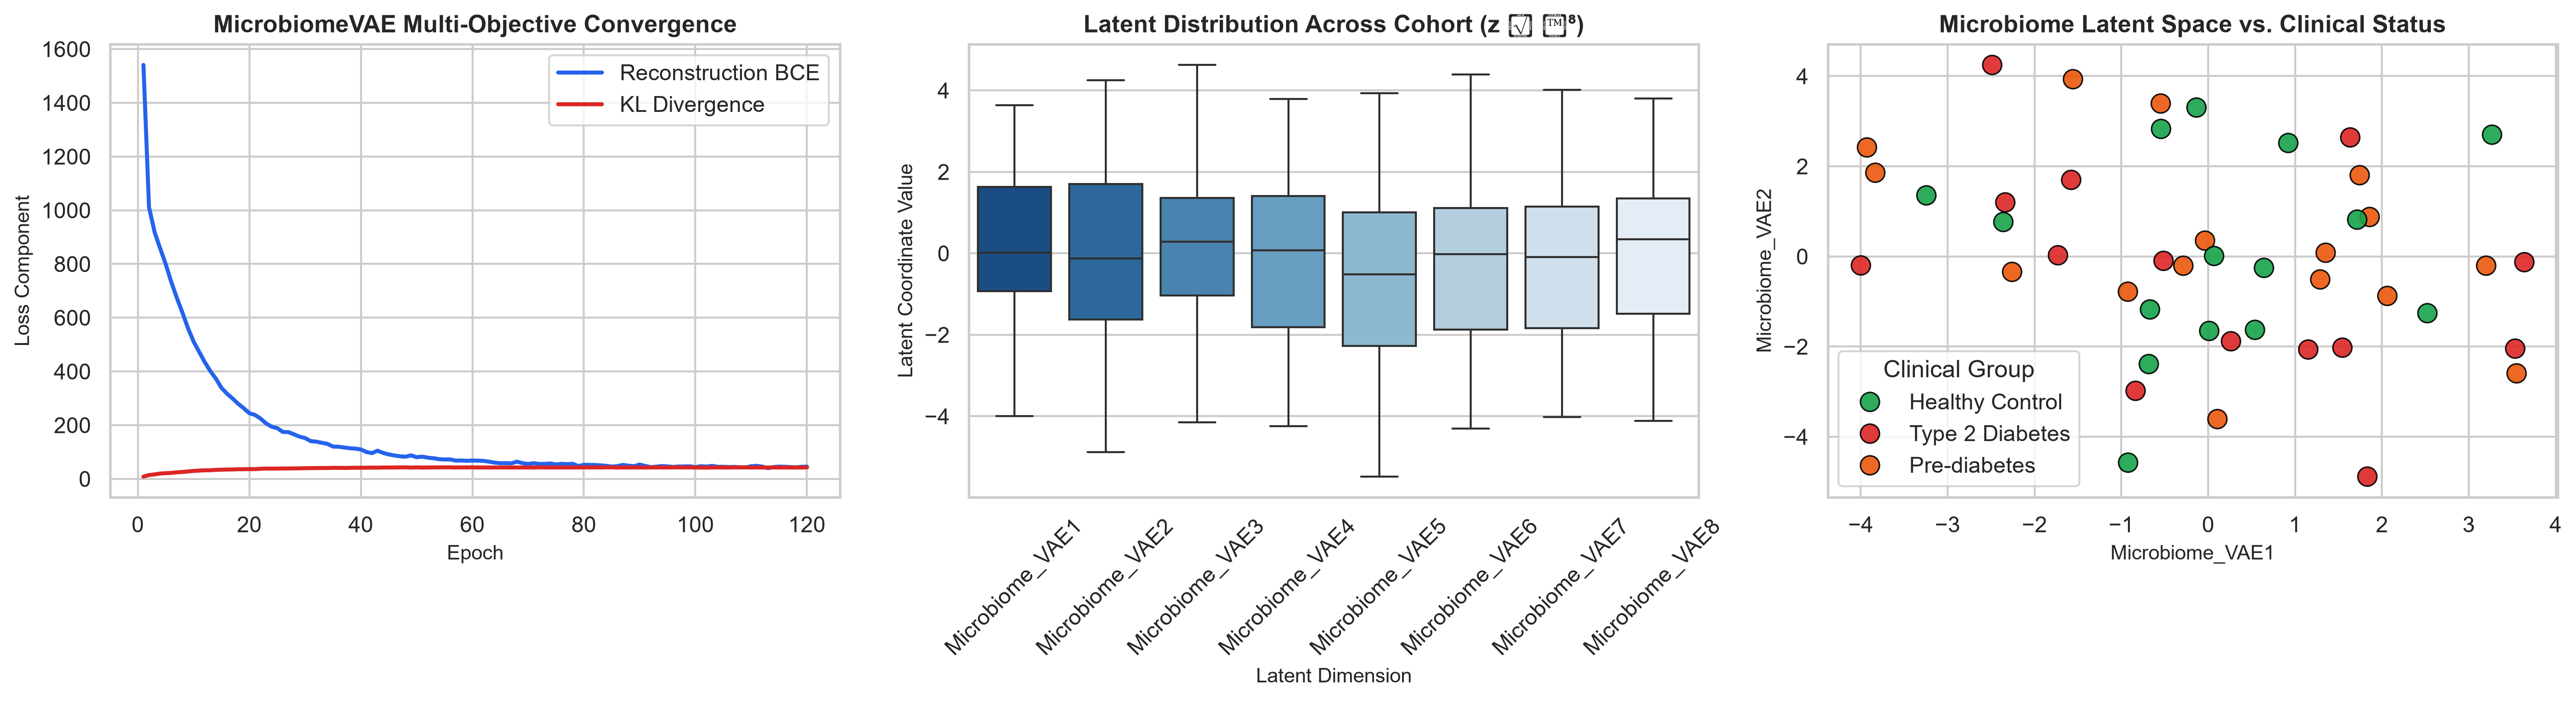
\includegraphics[width=\linewidth,height=0.65\textheight,keepaspectratio]{images/microbiome_vae_diagnostics.png}\\[0.1cm]
      {\scriptsize \color{DarkSlate} $\beta$-VAE training stability and reconstruction diagnostics}
    \end{column}
  \end{columns}
\end{frame}

% -----------------------------------------------------------------------------
% Slide 8: End-to-End System Architecture
% -----------------------------------------------------------------------------
\begin{frame}{GlycoTwin System Architecture}
  \centering
  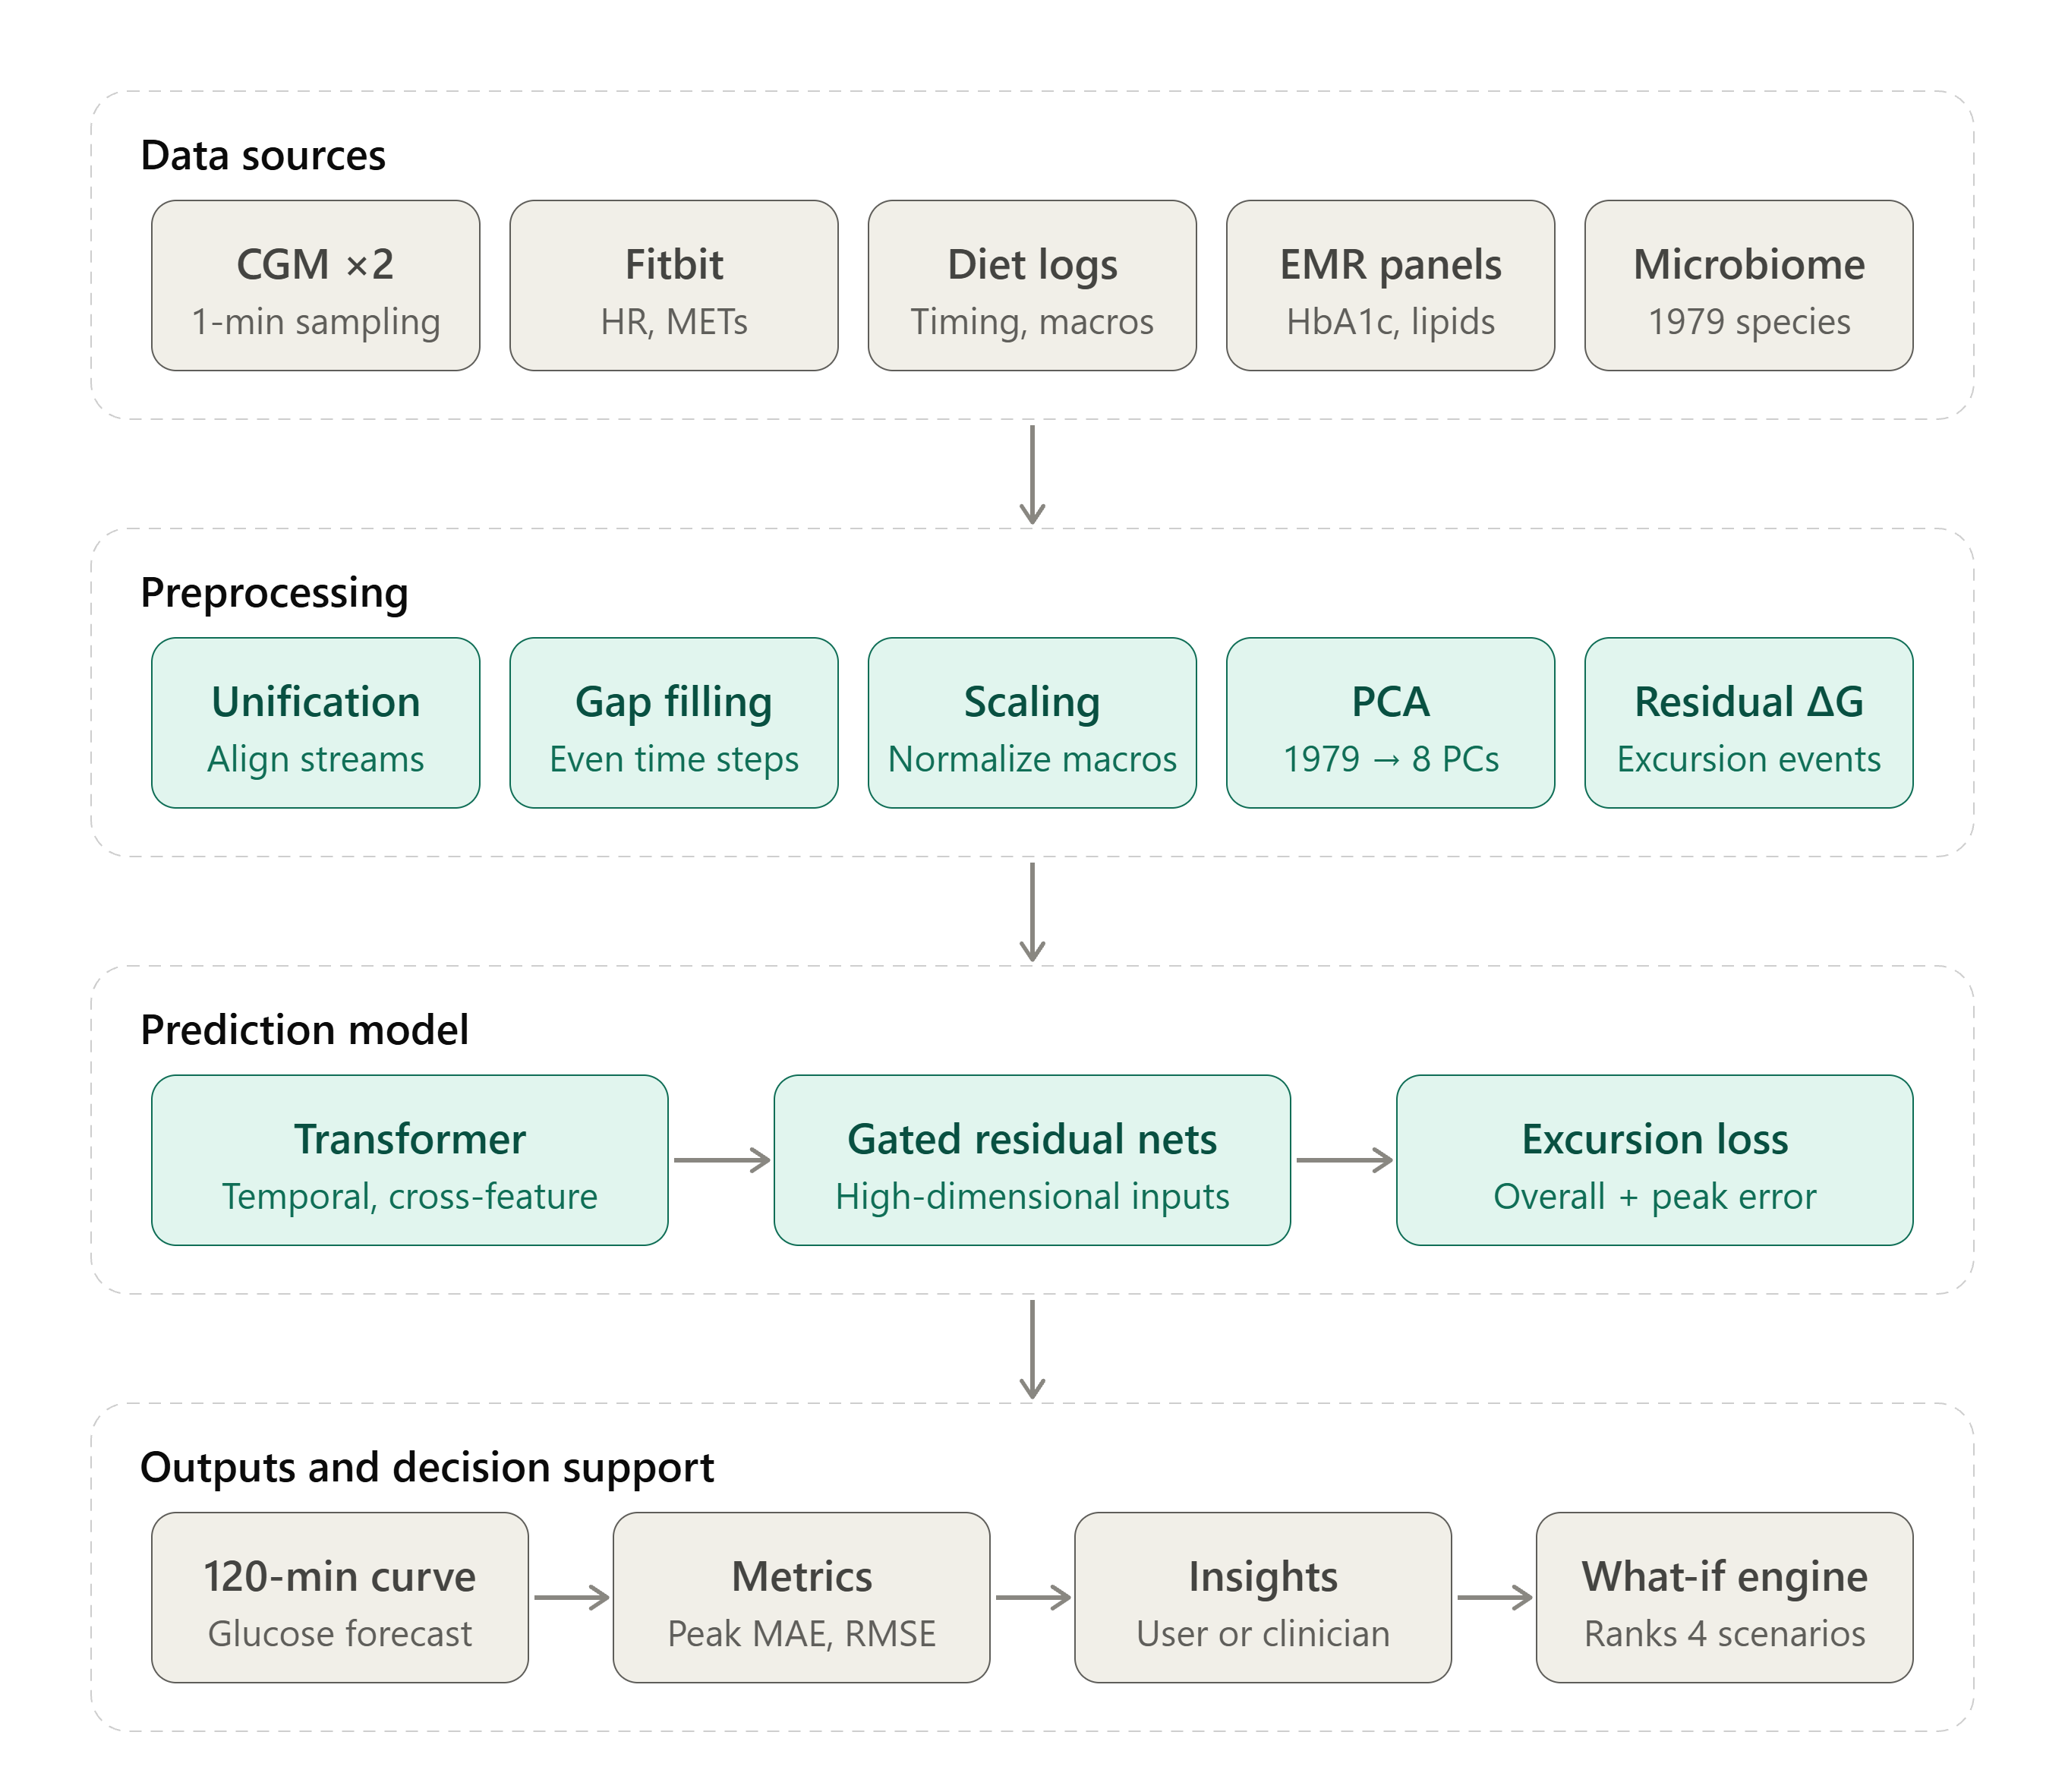
\includegraphics[width=0.92\textwidth,height=0.68\textheight,keepaspectratio]{images/t2d_digital_twin_architecture.png}
  
  \vspace{0.25cm}
  \begin{columns}[c]
    \begin{column}{0.32\textwidth}
      \centering {\footnotesize \textbf{\color{NavyBlue}1. Multi-Modal Inputs}}\\
      {\scriptsize CGM + Fitbit + Diet + Gut}
    \end{column}
    \begin{column}{0.34\textwidth}
      \centering {\footnotesize \textbf{\color{Teal}2. TransformerForecaster}}\\
      {\scriptsize Attention + Gated Static Fusion}
    \end{column}
    \begin{column}{0.32\textwidth}
      \centering {\footnotesize \textbf{\color{Crimson}3. What-If Simulator}}\\
      {\scriptsize Mobile Causal Lifestyle App}
    \end{column}
  \end{columns}
\end{frame}

% -----------------------------------------------------------------------------
% Slide 9: TransformerForecaster Model Design
% -----------------------------------------------------------------------------
\begin{frame}{TransformerForecaster: Dynamic \& Static Fusion}
  \begin{columns}[c]
    \begin{column}{0.48\textwidth}
      \begin{block}{Dynamic Pre-Meal Attention Encoder}
        \begin{itemize}\setlength{\itemsep}{0.4em}
          \item Takes 60-min pre-meal stream: Glucose, Heart Rate, and METs.
          \item 2-Layer Multi-Head Self-Attention ($h=4$ heads).
          \item Average temporal pooling captures pre-meal glucose trend and activity momentum.
        \end{itemize}
      \end{block}
    \end{column}
    
    \begin{column}{0.48\textwidth}
      \begin{block}{Gated Residual Network for Static Data}
        \begin{itemize}\setlength{\itemsep}{0.4em}
          \item Takes 61 static features (Nutrients, Labs, 8-D Gut VAE latents).
          \item Gating suppresses noisy biomarkers while amplifying key predictors (carbs, HOMA-IR).
        \end{itemize}
      \end{block}
    \end{column}
  \end{columns}
  
  \vspace{0.3cm}
  \begin{exampleblock}{\centering Output Head}
    \centering {\footnotesize Concatenates dynamic + static features $\to$ Predicts 24 time steps (5-min intervals over 2 hours).}
  \end{exampleblock}
\end{frame}

% -----------------------------------------------------------------------------
% Slide 10: Eliminating Baseline Bias & Smarter Loss
% -----------------------------------------------------------------------------
\begin{frame}{Eliminating Baseline Bias \& Composite Excursion Loss}
  \begin{columns}[c]
    \begin{column}{0.48\textwidth}
      \begin{block}{Residual Delta Target ($\Delta G$)}
        \begin{itemize}\setlength{\itemsep}{0.4em}
          \item Starting glucose varies widely ($85$ mg/dL healthy vs. $165$ mg/dL diabetic).
          \item We train the network on the \textbf{relative excursion rise}:
          $$\Delta G(t) = G(t) - G_0$$
          \item Eliminates baseline drift and prevents peak flattening.
        \end{itemize}
      \end{block}
    \end{column}
    
    \begin{column}{0.48\textwidth}
      \begin{block}{Composite Excursion Loss}
        \begin{itemize}\setlength{\itemsep}{0.4em}
          \item MSE alone rewards flat lines and misses sharp spikes.
          \item Our loss combines three objectives:
          \begin{enumerate}\setlength{\itemsep}{0.2em}
            \item Mean Squared Error (trajectory fit)
            \item Peak Error (penalizes missing maximum height)
            \item Slope Derivative Error (penalizes rise/fall rate)
          \end{enumerate}
        \end{itemize}
      \end{block}
    \end{column}
  \end{columns}
\end{frame}

% -----------------------------------------------------------------------------
% Slide 11: Experimental Protocol & Baselines
% -----------------------------------------------------------------------------
\begin{frame}{Experimental Setup: 5-Fold Group K-Fold Protocol}
  \begin{columns}[c]
    \begin{column}{0.50\textwidth}
      \begin{block}{Strictly Unseen Human Validation}
        \begin{itemize}\setlength{\itemsep}{0.5em}
          \item Random splitting causes data leakage because models memorize patient glucose baselines.
          \item We used \textbf{5-Fold Group K-Fold grouped by Subject ID}:
          \begin{itemize}\setlength{\itemsep}{0.2em}
            \item Train: 36 subjects ($\approx 1,306$ meals)
            \item Test: 9 completely unseen subjects ($\approx 327$ meals)
            \item Zero patient overlap between train and test.
          \end{itemize}
        \end{itemize}
      \end{block}
    \end{column}
    
    \begin{column}{0.48\textwidth}
      \begin{block}{Comparative Baselines Evaluated}
        \begin{enumerate}\setlength{\itemsep}{0.4em}
          \item \textbf{MLP Baseline:} Dense network with summary dynamic stats.
          \item \textbf{LSTM Forecaster:} 2-layer recurrent network.
          \item \textbf{GRU Forecaster:} 2-layer gated recurrent unit.
          \item \textbf{Transformer (PCA):} Transformer with 8 linear PCA features.
          \item \textbf{TransformerForecaster ($\beta$-VAE):} Our full model.
        \end{enumerate}
      \end{block}
    \end{column}
  \end{columns}
\end{frame}

% -----------------------------------------------------------------------------
% Slide 12: Benchmark Results
% -----------------------------------------------------------------------------
\begin{frame}{Quantitative Benchmarks on Unseen Participants}
  \begin{table}[!htbp]
  \centering
  \scriptsize
  \resizebox{\textwidth}{!}{%
  \begin{tabular}{llccccc}
  \toprule
  \textbf{Architecture} & \textbf{Modality Features} & \textbf{MAE (mg/dL)} & \textbf{RMSE (mg/dL)} & \textbf{$R^2$ Score} & \textbf{Clarke Safety (A+B)} \\
  \midrule
  MLP Baseline & Dynamic Summary + Static & 22.16 & 31.92 & 0.470 & 97.86\% \\
  LSTM Forecaster & 2-Layer LSTM + Static & 24.46 & 37.11 & 0.284 & 97.13\% \\
  GRU Forecaster & 2-Layer GRU + Static & 27.82 & 46.73 & -0.136 & 95.76\% \\
  \midrule
  Transformer (PCA) & MHSA + GRN + Linear PCA & 19.52 & 28.58 & 0.684 & 96.40\% \\
  \textbf{TransformerForecaster} & \textbf{MHSA + GRN + $\beta$-VAE} & \textbf{19.37} & \textbf{28.14} & \textbf{0.688} & \textbf{98.47\%} \\
  \midrule
  \emph{Literature Benchmark} & Gradient Boosted Decision Trees & 42.79 & --- & --- & --- \\
  \bottomrule
  \end{tabular}%
  }
  \end{table}

  \vspace{0.2cm}
  \begin{columns}[c]
    \begin{column}{0.32\textwidth}
      \begin{block}{\centering \textbf{30.4\% Error Drop}}
        {\scriptsize Substantially outperforms GRU baseline (27.82 $\to$ 19.37 mg/dL).}
      \end{block}
    \end{column}
    \begin{column}{0.34\textwidth}
      \begin{block}{\centering \textbf{54.7\% Gain vs. Literature}}
        {\scriptsize More than doubles accuracy of published CGMacros benchmark.}
      \end{block}
    \end{column}
    \begin{column}{0.32\textwidth}
      \begin{block}{\centering \textbf{68.8\% Variance Explained}}
        {\scriptsize $R^2 = 0.688$ across completely unseen human subjects.}
      \end{block}
    \end{column}
  \end{columns}
\end{frame}

% -----------------------------------------------------------------------------
% Slide 13: Trajectory Comparison Plots
% -----------------------------------------------------------------------------
\begin{frame}{Continuous Trajectory Forecast Visualizations}
  \begin{columns}[c]
    \begin{column}{0.52\textwidth}
      \centering
      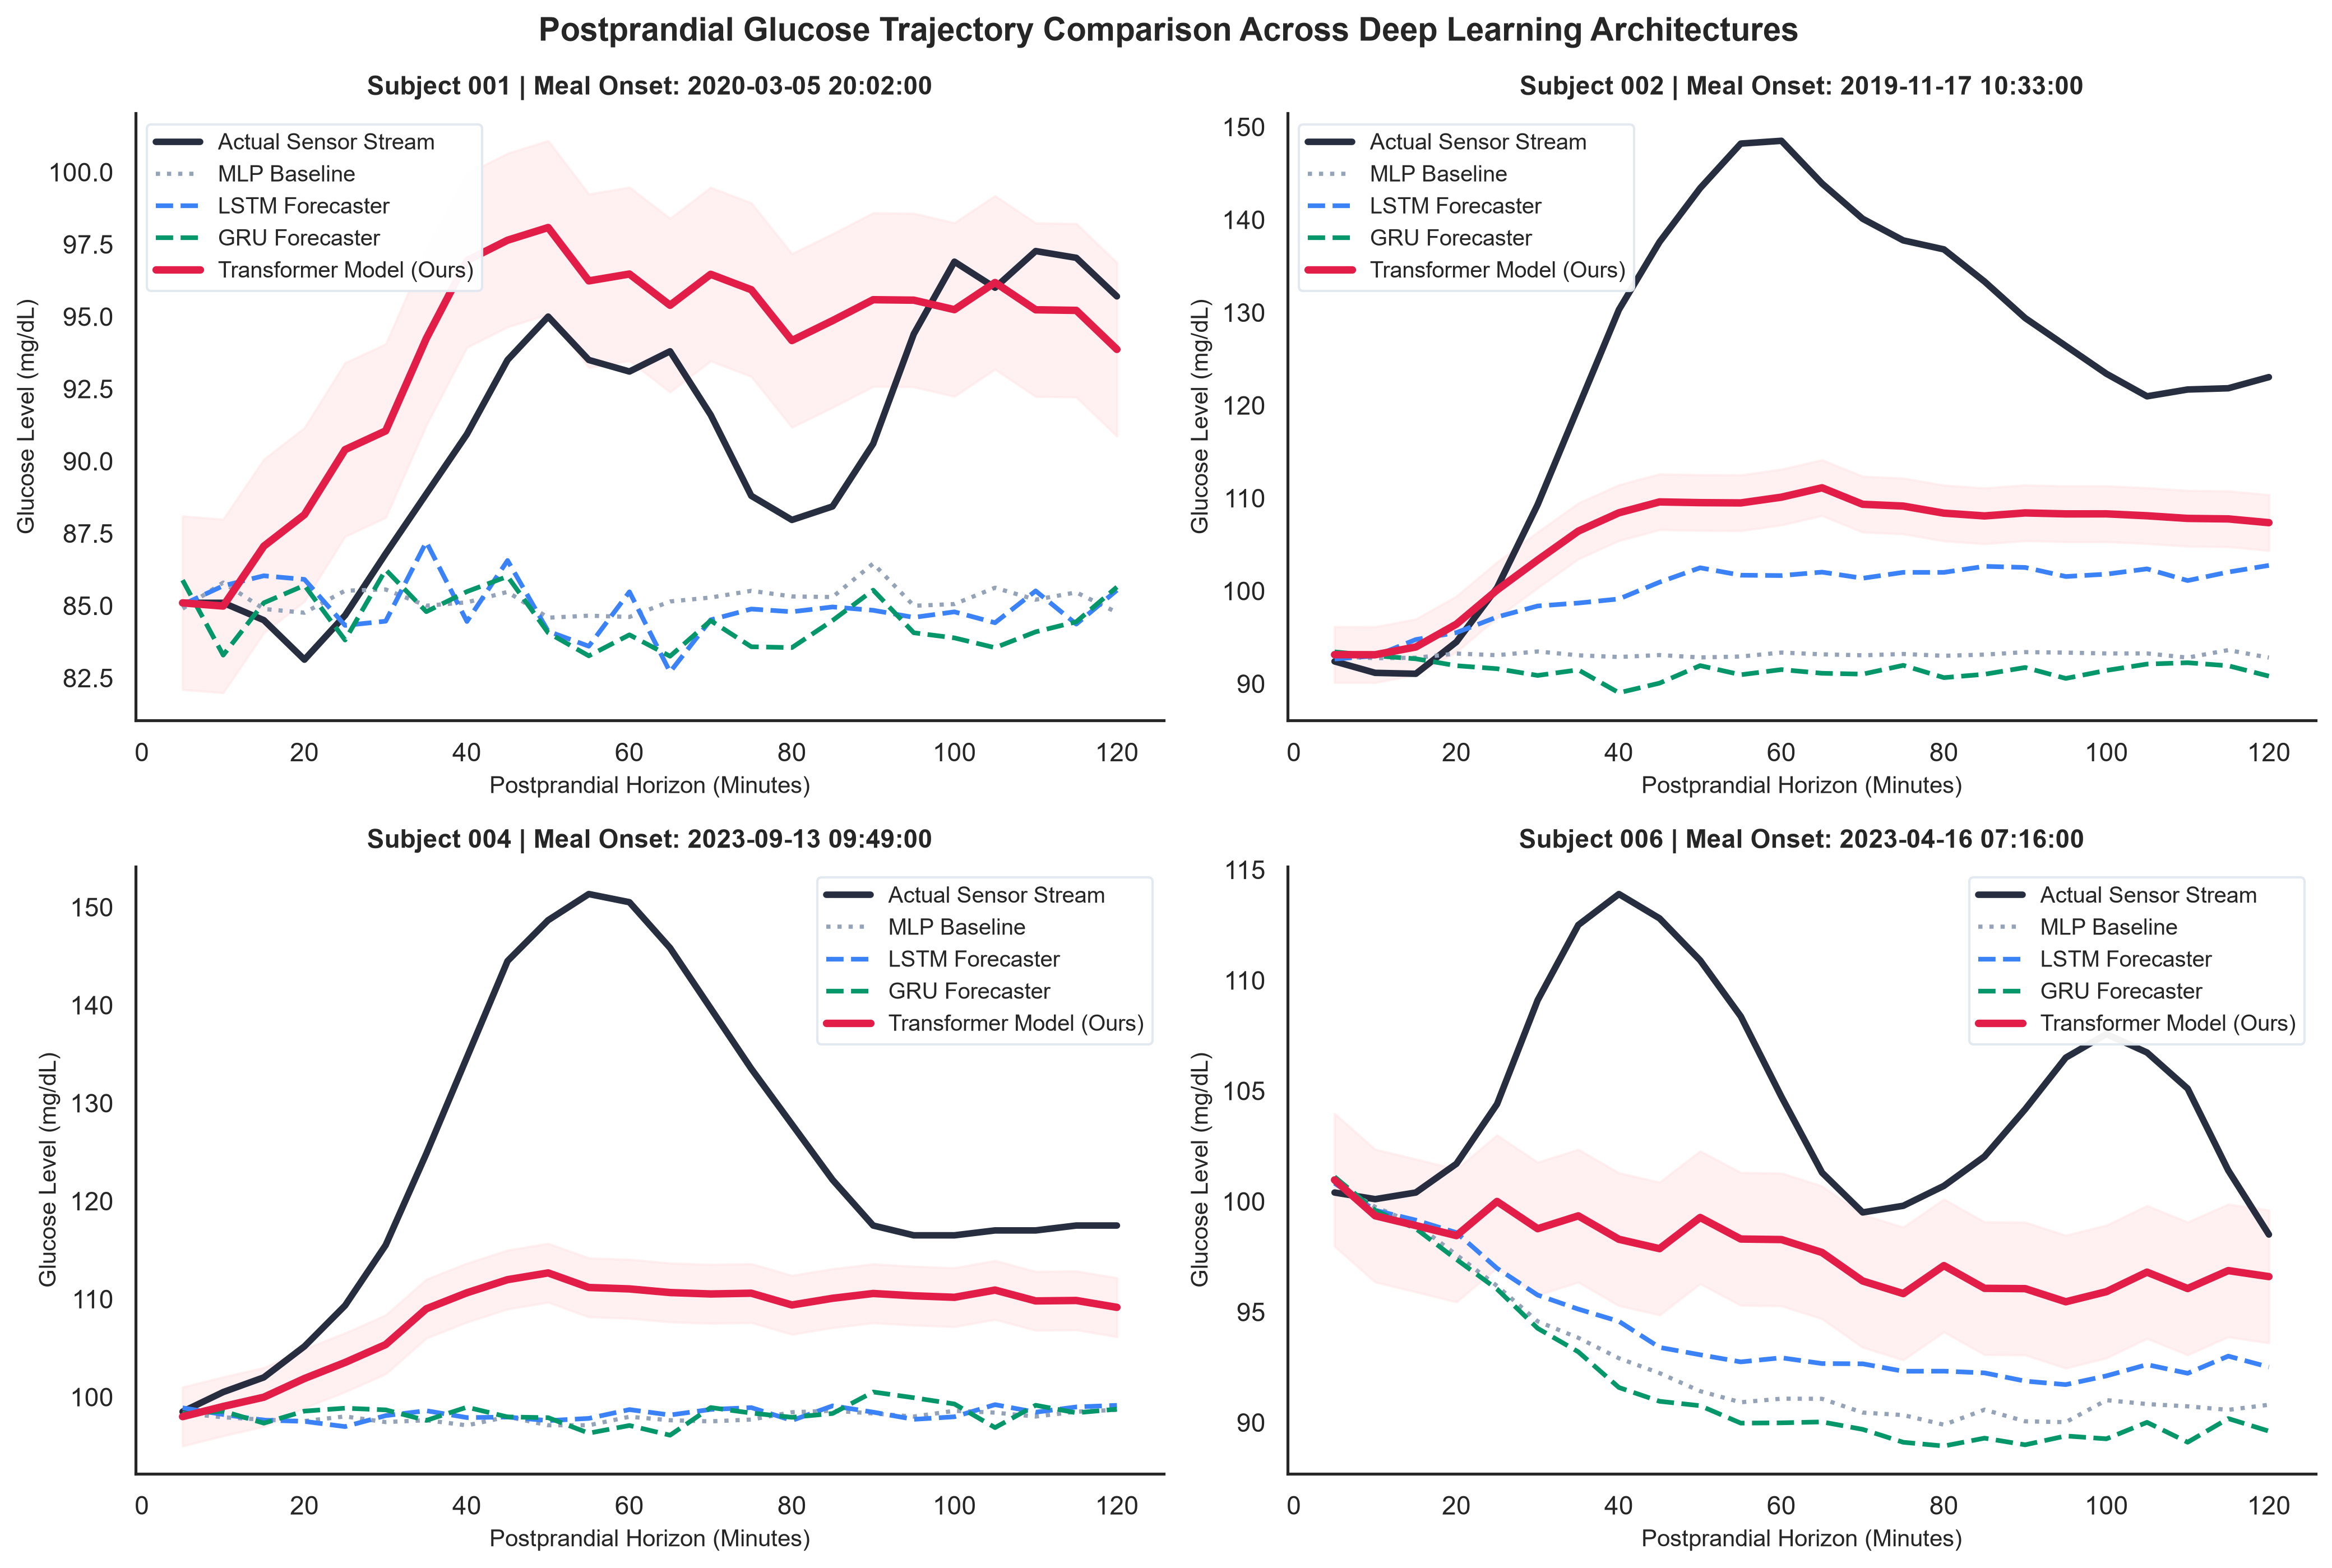
\includegraphics[width=\linewidth,height=0.70\textheight,keepaspectratio]{images/trajectory_comparison_all_models.png}
    \end{column}
    
    \begin{column}{0.45\textwidth}
      \begin{block}{Key Observations}
        \begin{itemize}\setlength{\itemsep}{0.6em}
          \item \textbf{Recurrent Models Flatten Peaks:} LSTM and GRU fail to capture acute rises, under-predicting dangerous spikes.
          \item \textbf{TransformerForecaster (Crimson):} Accurately follows the steep post-meal rise and peak amplitude.
          \item \textbf{Accurate Recovery:} Smoothly tracks clearance back to pre-meal levels without drift.
        \end{itemize}
      \end{block}
    \end{column}
  \end{columns}
\end{frame}

% -----------------------------------------------------------------------------
% Slide 14: Clinical Peak Excursion & Clarke Safety
% -----------------------------------------------------------------------------
\begin{frame}{Clinical Peak Accuracy \& Clarke Grid Safety}
  \begin{columns}[c]
    \begin{column}{0.48\textwidth}
      \begin{block}{Peak Spike \& Timing Accuracy}
        \begin{itemize}\setlength{\itemsep}{0.5em}
          \item \textbf{Peak Height MAE:} Reduced to \textbf{24.73 mg/dL} (12.8 mg/dL lower error than GRU).
          \item \textbf{Time-to-Peak ($T_{\max}$):} Error dropped from 31 minutes to \textbf{12.5 minutes}.
          \item Accurately predicts \emph{when} and \emph{how high} glucose will peak.
        \end{itemize}
      \end{block}
    \end{column}
    
    \begin{column}{0.48\textwidth}
      \begin{exampleblock}{Clarke Error Grid Clinical Safety}
        \begin{itemize}\setlength{\itemsep}{0.5em}
          \item \textbf{98.47\%} of forecasts fall in \textbf{Zones A and B} (Clinically safe for treatment decisions).
          \item \textbf{0.00\%} in dangerous error \textbf{Zones D or E}.
          \item Meets international regulatory medical criteria (ISO 15197).
        \end{itemize}
      \end{exampleblock}
    \end{column}
  \end{columns}
\end{frame}

% -----------------------------------------------------------------------------
% Slide 15: Causal What-If Simulation Engine
% -----------------------------------------------------------------------------
\begin{frame}{From Prediction to Action: Causal What-If Simulation}
  \begin{columns}[c]
    \begin{column}{0.50\textwidth}
      \begin{block}{Simulating 4 Pre-Meal Scenarios}
        Before eating, the engine simulates 4 lifestyle options:
        \begin{enumerate}\setlength{\itemsep}{0.3em}
          \item \textbf{Planned Meal:} Baseline control.
          \item \textbf{-50\% Carbs:} Portion control / substitution.
          \item \textbf{+30m Walk:} Immediate light post-meal walk.
          \item \textbf{Dual Action:} Carb reduction + 30-min walk.
        \end{enumerate}
      \end{block}
    \end{column}
    
    \begin{column}{0.48\textwidth}
      \begin{exampleblock}{Clinical Utility Score ($U \in [0, 1]$)}
        Ranks scenarios based on:
        \begin{itemize}\setlength{\itemsep}{0.3em}
          \item \% Time-in-Range ($70 - 180$ mg/dL)
          \item Maximum peak glucose penalty
          \item Rate of rise penalty
        \end{itemize}
        {\footnotesize Green badge ($U \ge 0.85$) indicates optimal safety.}
      \end{exampleblock}
    \end{column}
  \end{columns}
\end{frame}

% -----------------------------------------------------------------------------
% Slide 16: Case Study: Subject 011
% -----------------------------------------------------------------------------
\begin{frame}{Clinical Case Study: Subject 011 Analysis}
  \begin{columns}[c]
    \begin{column}{0.50\textwidth}
      \centering
      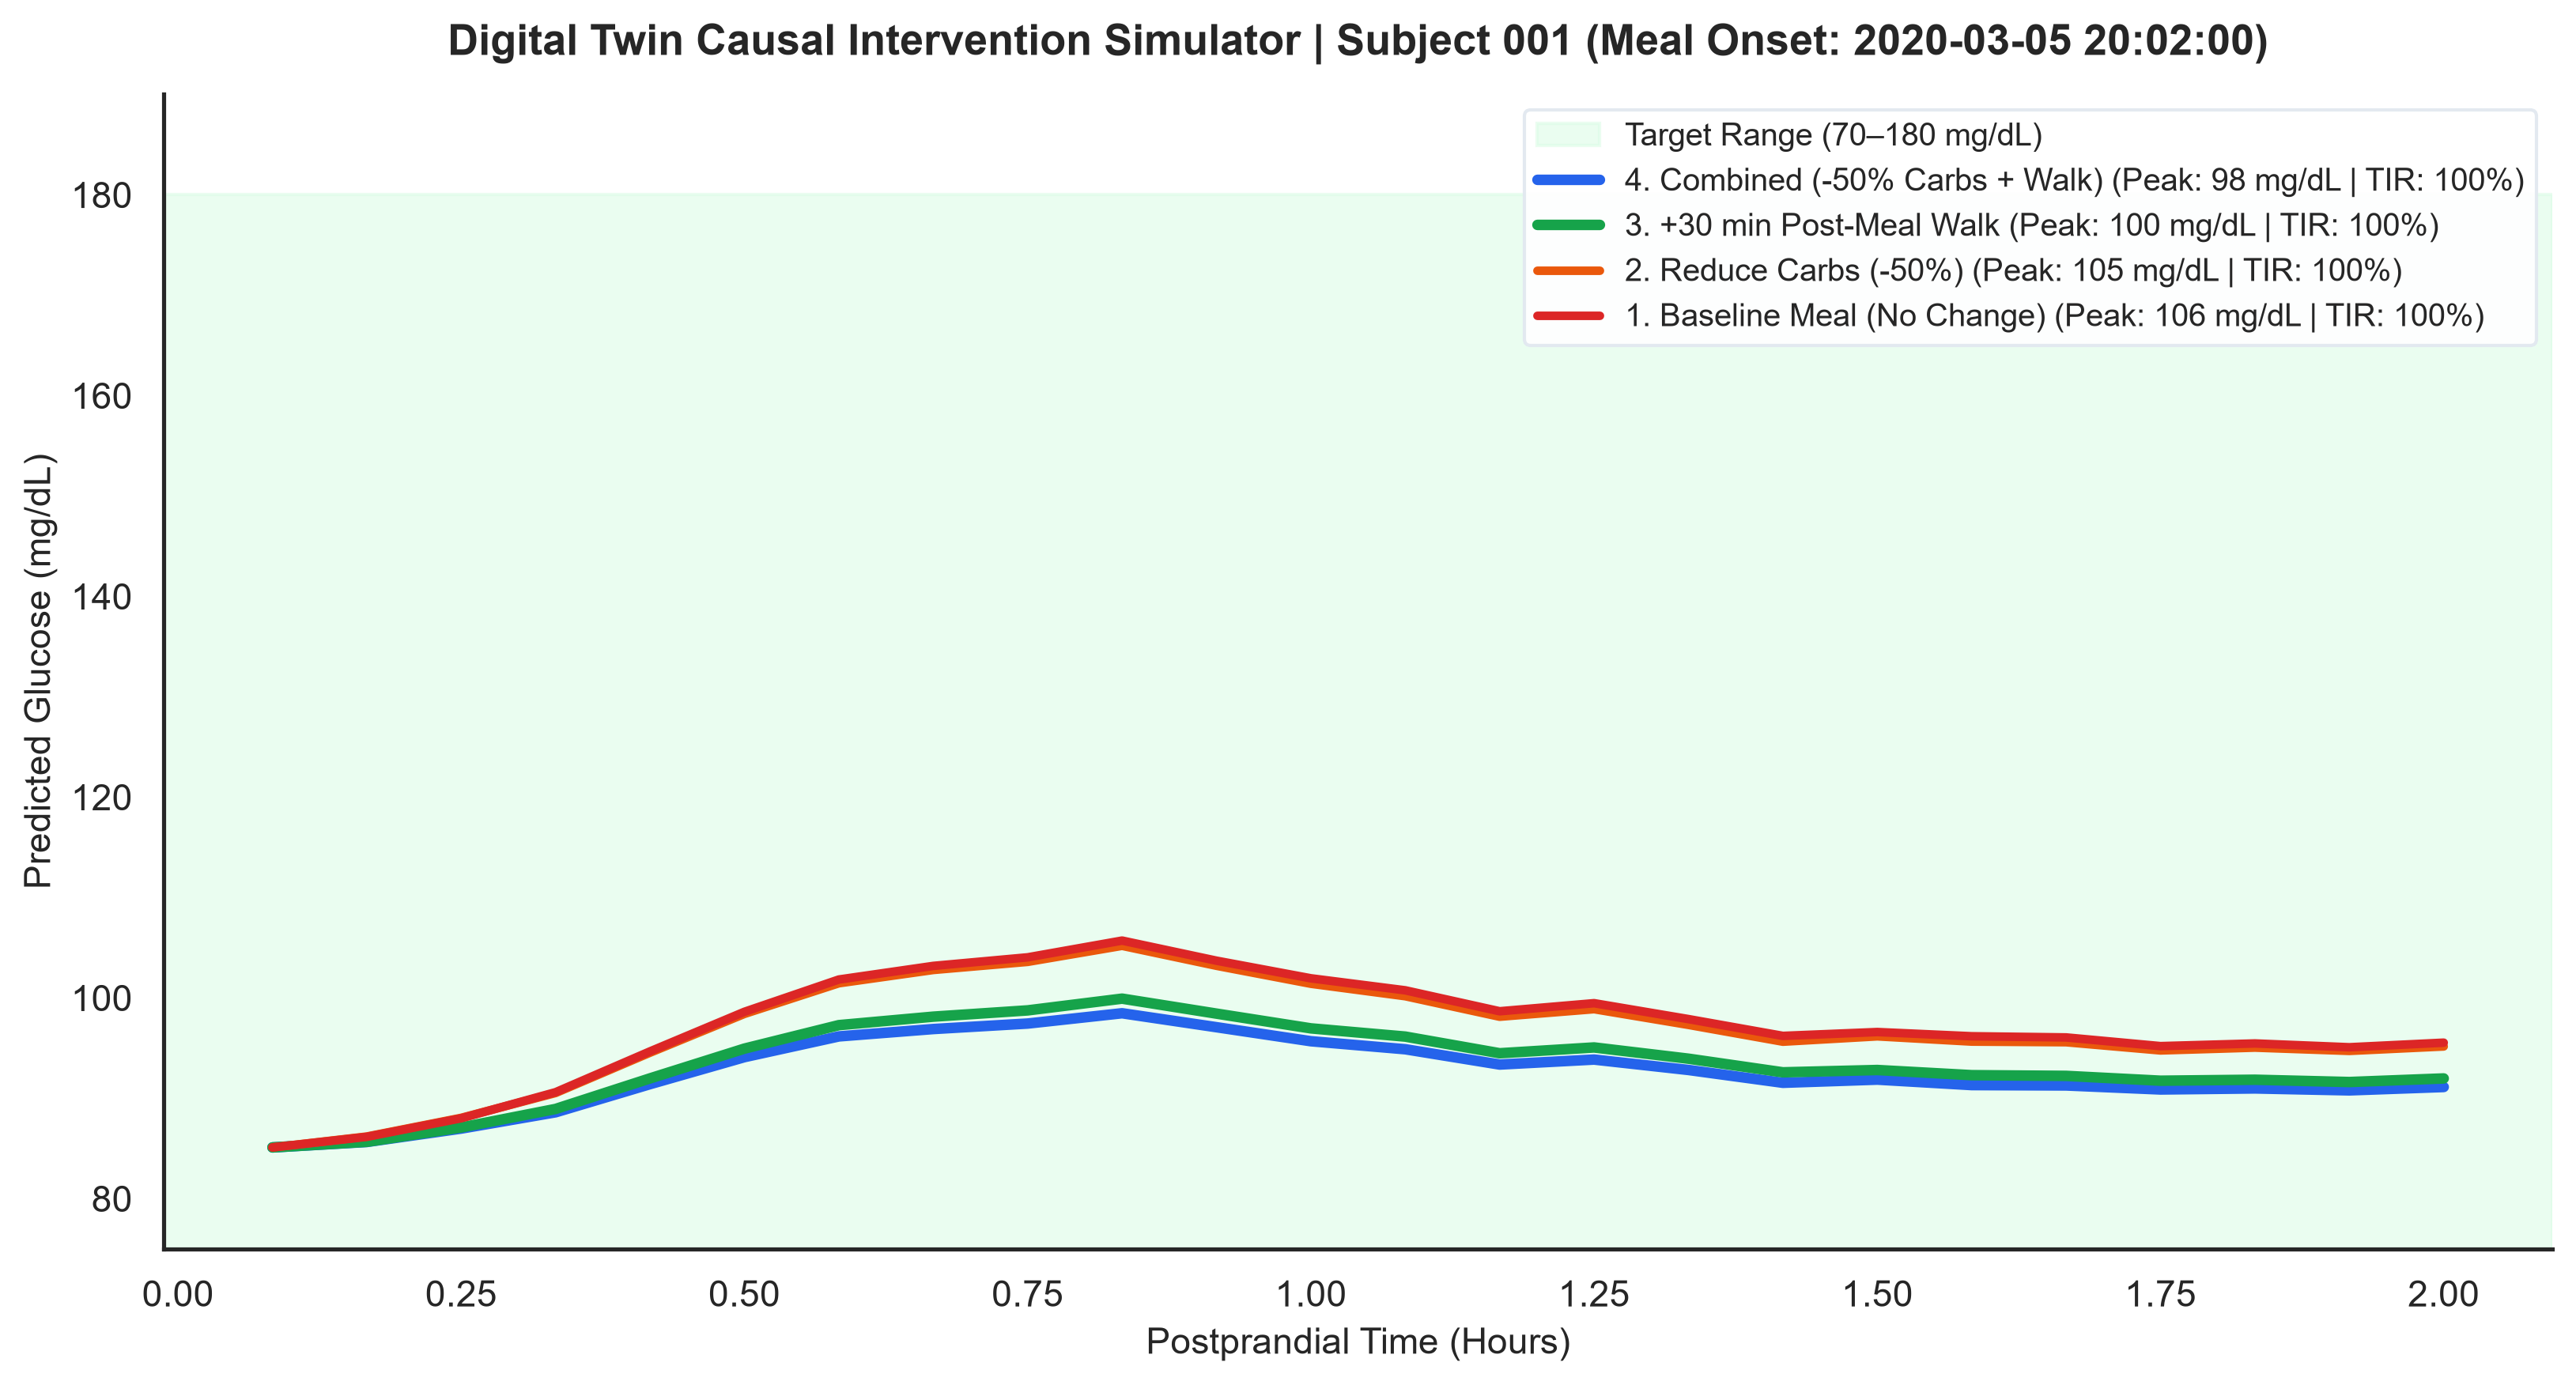
\includegraphics[width=\linewidth,height=0.68\textheight,keepaspectratio]{images/causal_simulator_trajectories.png}\\[0.1cm]
      {\scriptsize \color{DarkSlate} Simulated intervention curves against 70--180 mg/dL target}
    \end{column}
    
    \begin{column}{0.48\textwidth}
      \begin{block}{Intervention Comparison}
        \begin{itemize}\setlength{\itemsep}{0.4em}
          \item \textbf{Planned Meal:} Spikes by \textbf{+48.2 mg/dL} to 168.2 mg/dL ($U = 0.748$).
          \item \textbf{-50\% Carbs:} Blunts rise to \textbf{+24.1 mg/dL} ($U = 0.842$).
          \item \textbf{+30m Walk:} Blunts rise to \textbf{+18.6 mg/dL} ($U = 0.865$).
          \item \textbf{Combined:} Reduces excursion rise to just \textbf{+6.3 mg/dL} ($\mathbf{U = 0.932}$, Rank 1).
        \end{itemize}
      \end{block}
    \end{column}
  \end{columns}
\end{frame}

% -----------------------------------------------------------------------------
% Slide 17: GlycoTwin Mobile Web App
% -----------------------------------------------------------------------------
\begin{frame}{Mobile-First Progressive Web App (GlycoTwin)}
  \begin{columns}[c]
    \begin{column}{0.28\textwidth}
      \centering
      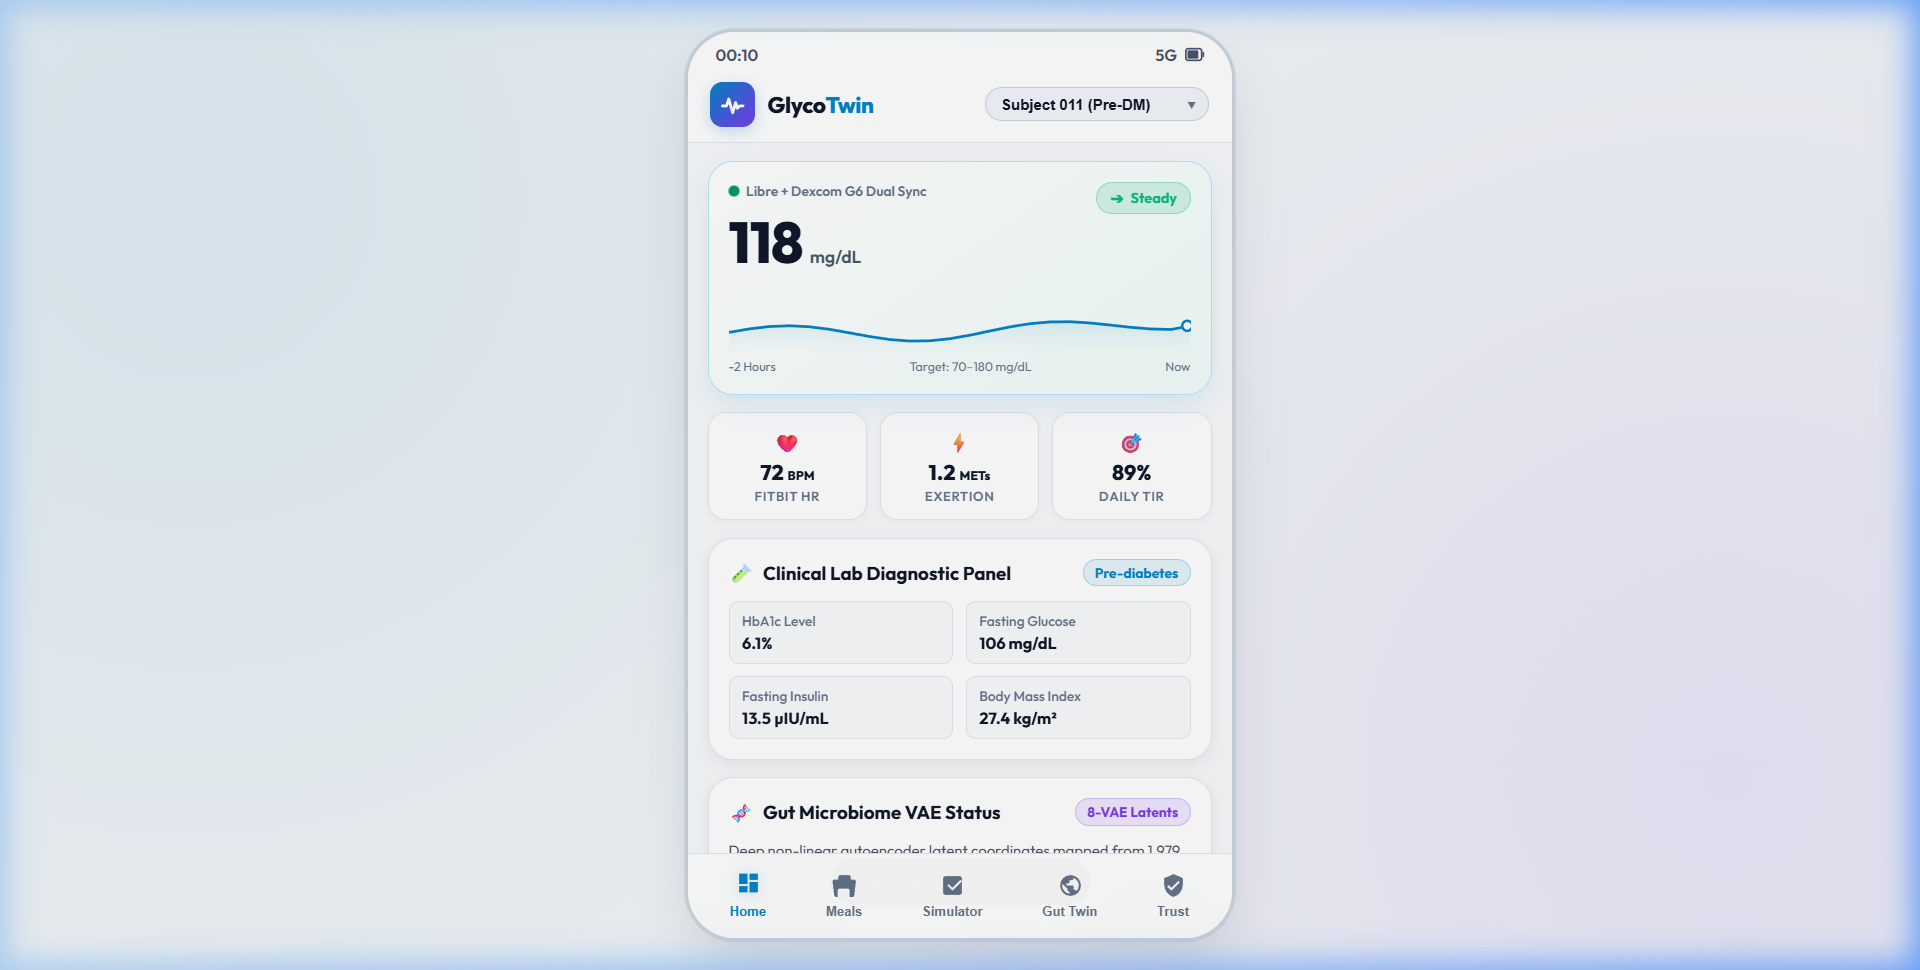
\includegraphics[width=0.92\linewidth,height=0.65\textheight,keepaspectratio]{images/mobile_dashboard_preview.png}\\[0.05cm]
      {\scriptsize Telemetry Dashboard}
    \end{column}
    
    \begin{column}{0.28\textwidth}
      \centering
      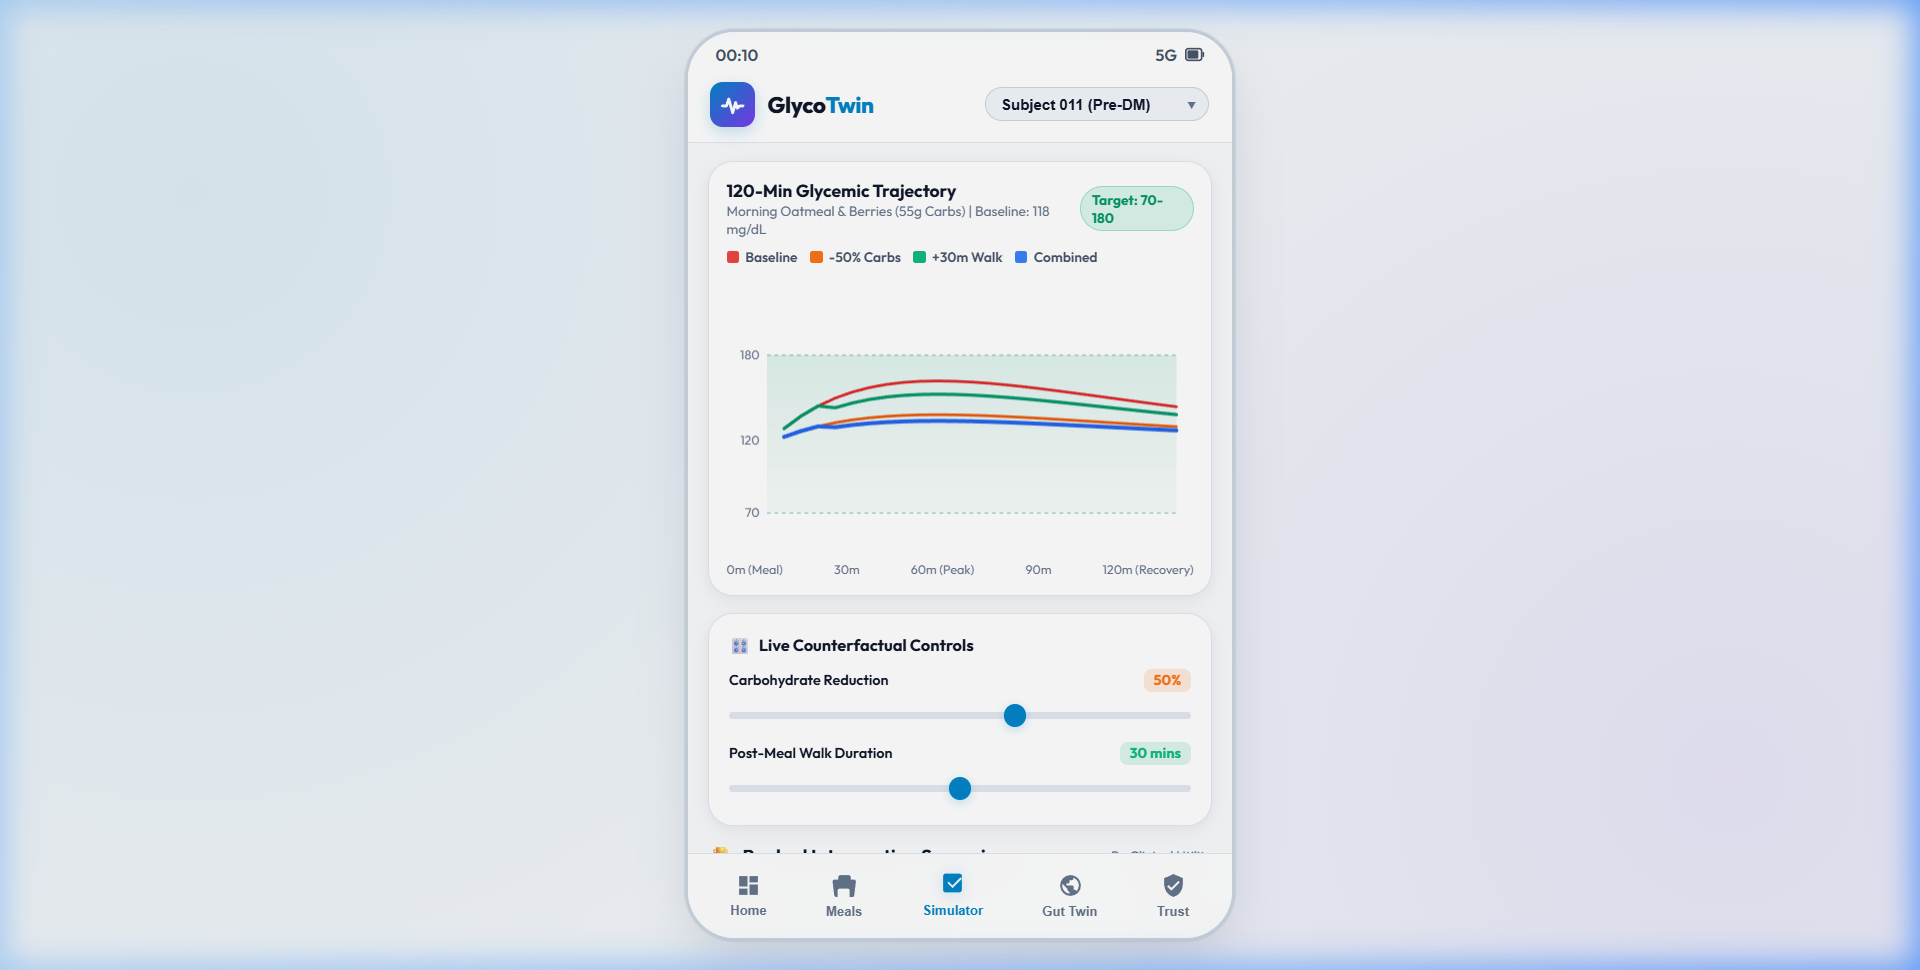
\includegraphics[width=0.92\linewidth,height=0.65\textheight,keepaspectratio]{images/mobile_simulator_preview.png}\\[0.05cm]
      {\scriptsize Causal Simulator}
    \end{column}
    
    \begin{column}{0.42\textwidth}
      \begin{block}{Key App Features}
        \begin{itemize}\setlength{\itemsep}{0.5em}
          \item \textbf{Lightweight Frontend:} Built with Vanilla HTML5/CSS/JS (no heavy frameworks, $<100$ms load).
          \item \textbf{Touch Sliders:} Instantly adjust meal carbs, fiber, protein, and walk duration.
          \item \textbf{Interactive Canvas:} Drag finger across the 2-hour forecasted curve.
        \end{itemize}
      \end{block}
    \end{column}
  \end{columns}
\end{frame}

% -----------------------------------------------------------------------------
% Slide 18: Summary of Contributions
% -----------------------------------------------------------------------------
\begin{frame}{Summary of Key Contributions}
  \begin{columns}[c]
    \begin{column}{0.48\textwidth}
      \begin{block}{1. Synchronized Multi-Modal Data}
        Aligned dual CGM, smartwatch exertion, meal nutrition, clinical labs, and 1,979 gut taxa.
      \end{block}
      
      \vspace{0.2cm}
      \begin{block}{2. Deep Microbiome $\beta$-VAE}
        Compressed 1,979 sparse bacteria into 8 continuous latents with 1.0000 ROC-AUC.
      \end{block}
    \end{column}
    
    \begin{column}{0.48\textwidth}
      \begin{block}{3. TransformerForecaster}
        Eliminated baseline offset bias; achieved \textbf{19.37 mg/dL MAE} on unseen patients (30.4\% better than GRU).
      \end{block}
      
      \vspace{0.2cm}
      \begin{block}{4. Causal Mobile Simulation}
        Shifted diabetes care from reactive alerts to pre-meal proactive lifestyle decisions (98.47\% Clarke safety).
      \end{block}
    \end{column}
  \end{columns}
\end{frame}

% -----------------------------------------------------------------------------
% Slide 19: Limitations & Future Scope
% -----------------------------------------------------------------------------
\begin{frame}{Limitations \& Future Research Directions}
  \begin{columns}[c]
    \begin{column}{0.48\textwidth}
      \begin{alertblock}{Limitations}
        \begin{itemize}\setlength{\itemsep}{0.5em}
          \item \textbf{Meal Logging Noise:} Portion estimates in free-living logs have small subjective bias.
          \item \textbf{CGM Sensor Delay:} 5--10 minute physiological delay in interstitial fluid.
          \item \textbf{Cohort Diversity:} Evaluated on 45 Portuguese participants; broader multi-center trials needed.
        \end{itemize}
      \end{alertblock}
    \end{column}
    
    \begin{column}{0.48\textwidth}
      \begin{exampleblock}{Future Work}
        \begin{itemize}\setlength{\itemsep}{0.5em}
          \item \textbf{Conformal Prediction:} Add 95\% confidence bands around curves for uncertainty estimation.
          \item \textbf{Smart Insulin Pens:} Connect forecasts to smart pens for automated pre-meal dosing.
          \item \textbf{Longitudinal Gut Tracking:} Update digital twin as gut flora shifts over months of diet changes.
        \end{itemize}
      \end{exampleblock}
    \end{column}
  \end{columns}
\end{frame}

% -----------------------------------------------------------------------------
% Slide 20: Conclusion & Q&A
% -----------------------------------------------------------------------------
\begin{frame}[plain]
  \begin{center}
    \vspace{0.6cm}
    
\includegraphics[height=1.25cm]{images/univA.png}\\[0.25cm]
    {\LARGE \textbf{\color{NavyBlue} Thank You!}}\\[0.2cm]
    {\small \color{Teal} Questions \& Discussion}\\[0.4cm]
    
    \begin{block}{\centering Project Repository}
      \centering \footnotesize
      \textbf{GitHub:} \href{https://github.com/AoD-X-abhi/GlycoTwin-T2DM}{\color{NavyBlue}\texttt{https://github.com/AoD-X-abhi/GlycoTwin-T2DM}}
    \end{block}
    
    \vspace{0.4cm}
    {\footnotesize \textbf{Department of Artificial Intelligence} $\cdot$ Amrita Vishwa Vidyapeetham}\\
    \vspace{0.15cm}
    {\scriptsize \textbf{Guide:} Dr. Keerthika K \quad $\vert$ \quad \textbf{Authors:} Divagar S, Abhishek Pandey, Prem}
  \end{center}
\end{frame}

\end{document}
